\documentclass[]{cv-style} % Add 'print' in [] to get print-view
\usepackage{graphicx}
\begin{document}
\header{Ashin}{Asok}
\begin{aside}
\section{.}
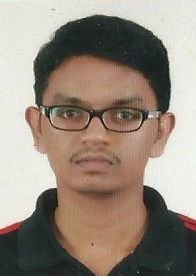
\includegraphics[width=4cm]{Scan.jpeg}
\section{Contact}
Ashin Nivas
Elamakkara
Kochi-682026
~
+91 9895346651
+91 7293146180
~
ashin9895@gmail.com
\section{Languages}
English
Hindi
Malayalam
\section{Tools}
Prezi
MS Office
iMovie
Final Cut Pro
Keynote
Adobe After Effects
\end{aside}
\section{Career Objective}
  \vspace{-0.2cm}
Looking for a career to show the best of my professional ability, analytic skills and techniques to enhance my knowledge as well as contribute to my organization to the best of my potential.

\section{Education}
\begin{entrylist}
\entry
{2013 - 2017}
{B.Tech. {\normalfont in Computer Science and Engineering [59.68\%]}}
{Kalamassery, Kochi}
{Albertian Institute of Science and Technology}
\entry
{2012 - 2013}
{H.S.C. {\normalfont in Computer Science [67.2\%]}}
{Naval Base, Kochi}
{Kendriya Vidyalaya No 1}
\entry
{2010 - 2011}
{S.S.C. {\normalfont in Computer Science [8.2 out of 10]}}
{Naval Base, Kochi}
{Kendriya Vidyalaya No 1}
\end{entrylist} 

\section{Projects Undertaken}
\begin{entrylist}
\entry
  {2016 - Now}
  {Open Information Extraction and Relation Extraction}
  {AISAT}
  {\jobtitle{Main Project}\\
Open  IE ,  a  new  extraction paradigm where the system makes a single data-driven pass over its corpus and extracts a large set of relational tuples without requiring any human input.}

\entry
  {2015 - 2016}
  {Natural Language Processing using Python and Django}
  {AISAT}
  {\jobtitle{Mini Project}\\
By definition, the natural language search system is a system which will retrieve the most appropriate documents for the user by ranking the documents. This system will apply Information Retrieval to retrieve the documents and appropriate matching sentences from the document.}

\end{entrylist}
\section{Skills}
\begin{entrylist}
\entry
{Software Languages : }
{     C/C++ , Python , Swift , Java , PHP , Perl}
{}
{}
\entry
{Web Technologies : }
{     Django , Ajax}
{}
{}
\entry
{Operating Systems :}
{     MacOS , Linux , Windows}
{}
{}
\end{entrylist}
\section{Extra Curricular Activities}
\begin{entrylist}
\entry
{2016}
{Esperanza}
{}
{Volunteer and Incharge of Main Coding Event- Code-A-thon .}
\entry
{2015}
{Intra College Arts Fest}
{}
{Won Second prize for Poetry Writing}
\entry
{2015}
{Discover Thinking Quiz}
{}
{Volunteer for the event conducted by Computer Society of India}
\entry
{2014}
{Excel 2k14}
{}
{Participated in Coding Event conducted by Model Engineering college}
\entry
{2012}
{District Level Science Fair}
{}
{Selected for the Project titled " Maximum Range of Projectile Motion ".}
\end{entrylist}
\end{document}